% Options for packages loaded elsewhere
\PassOptionsToPackage{unicode}{hyperref}
\PassOptionsToPackage{hyphens}{url}
%
\documentclass[
  italian,
]{article}
\usepackage{amsmath,amssymb}
\usepackage{lmodern}
\usepackage{iftex}
\usepackage{geometry}
\headsep = -20pt
\textheight = 719pt
\footskip = -10pt
\usepackage{subfig}
\ifPDFTeX
  \usepackage[T1]{fontenc}
  \usepackage[utf8]{inputenc}
  \usepackage{textcomp} % provide euro and other symbols
\else % if luatex or xetex
  \usepackage{unicode-math}
  \defaultfontfeatures{Scale=MatchLowercase}
  \defaultfontfeatures[\rmfamily]{Ligatures=TeX,Scale=1}
\fi
% Use upquote if available, for straight quotes in verbatim environments
\IfFileExists{upquote.sty}{\usepackage{upquote}}{}
\IfFileExists{microtype.sty}{% use microtype if available
  \usepackage[]{microtype}
  \UseMicrotypeSet[protrusion]{basicmath} % disable protrusion for tt fonts
}{}
\makeatletter
\@ifundefined{KOMAClassName}{% if non-KOMA class
  \IfFileExists{parskip.sty}{%
    \usepackage{parskip}
  }{% else
    \setlength{\parindent}{0pt}
    \setlength{\parskip}{6pt plus 2pt minus 1pt}}
}{% if KOMA class
  \KOMAoptions{parskip=half}}
\makeatother
\usepackage{xcolor}
\IfFileExists{xurl.sty}{\usepackage{xurl}}{} % add URL line breaks if available
\IfFileExists{bookmark.sty}{\usepackage{bookmark}}{\usepackage{hyperref}}
\hypersetup{
  pdftitle={Progetto Matlab},
  pdfauthor={Mattia Maglie 1189315; Francesco Marcato 1189319; Marco Martini 1189321},
  pdflang={it-IT},
  hidelinks,
  pdfcreator={LaTeX via pandoc}}
\urlstyle{same} % disable monospaced font for URLs
\usepackage{listings}
\newcommand{\passthrough}[1]{#1}
\lstset{defaultdialect=[5.3]Lua}
\lstset{defaultdialect=[x86masm]Assembler}
\usepackage{graphicx}
\makeatletter
\def\maxwidth{\ifdim\Gin@nat@width>\linewidth\linewidth\else\Gin@nat@width\fi}
\def\maxheight{\ifdim\Gin@nat@height>\textheight\textheight\else\Gin@nat@height\fi}
\makeatother
% Scale images if necessary, so that they will not overflow the page
% margins by default, and it is still possible to overwrite the defaults
% using explicit options in \includegraphics[width, height, ...]{}
\setkeys{Gin}{width=\maxwidth,height=\maxheight,keepaspectratio}
% Set default figure placement to htbp
\makeatletter
\def\fps@figure{htbp}
\makeatother
\setlength{\emergencystretch}{3em} % prevent overfull lines
\providecommand{\tightlist}{%
  \setlength{\itemsep}{0pt}\setlength{\parskip}{0pt}}
\setcounter{secnumdepth}{-\maxdimen} % remove section numbering
\ifXeTeX
  % Load polyglossia as late as possible: uses bidi with RTL langages (e.g. Hebrew, Arabic)
  \usepackage{polyglossia}
  \setmainlanguage[]{italian}
\else
  \usepackage[main=italian]{babel}
% get rid of language-specific shorthands (see #6817):
\let\LanguageShortHands\languageshorthands
\def\languageshorthands#1{}
\fi
\ifLuaTeX
  \usepackage{selnolig}  % disable illegal ligatures
\fi

\title{Progetto Matlab}
\usepackage{etoolbox}
\makeatletter
\providecommand{\subtitle}[1]{% add subtitle to \maketitle
  \apptocmd{\@title}{\par {\large #1 \par}}{}{}
}
\makeatother
\subtitle{Depth Map per ridurre falsi positivi in Face Detection}
\author{Mattia Maglie 1189315 \and Francesco Marcato 1189319 \and Marco
Martini 1189321}
\date{}

\begin{document}
\maketitle

\hypertarget{descrizione-metodo}{%
\section{Descrizione Metodo}\label{descrizione-metodo}}

\hypertarget{descrizione-testuale}{%
\subsection{Descrizione Testuale}\label{descrizione-testuale}}

Data la matrice DepthDATA, considero per ogni elemento il campo (di
indice 2) contenente la matrice di valori di profondità. Richiamo quindi
il metodo ``FixMatrix'' che va a sostituire nella matrice di profondità
i valori 0 con il massimo delle profondità presenti nella matrice. I
valori a 0 di Depth infatti, indicano un ``errore'' nella determinazione
della profondità da parte del sensore; nella maggior parte dei casi
l'errore è causato da elementi troppo lontani dal sensore.\\
Per questo vengono posizionati sulla massima profondità, ovvero sullo
``sfondo''.

Dalla matrice modificata viene poi presa la riga centrale, e si effettua
una ``regressione parabolica'' sui valori della riga centrale. Per la
regressione parabolica si usa la funzione fit del Curve Fitting Toolbox.

I coefficienti vengono poi usati per calcolare la posizione in ascissa
del vertice.

Definisco due margini calcolati come segue:

\(A = matrixHCenter - marginRate \cdot matrixWidth\)

\(B = matrixHCenter + marginRate \cdot matrixWidth\)

Dove \(matrixHCenter\) è la posizione della colonna centrale della
matrice di profondità e \(matrixWidth\) è la larghezza della matrice.

Il coefficiente marginRate arbitrario che indica quanto ci si distanzia
dal centro della matrice nel considerare i margini.

Nel caso in cui il vertice della parabola ottenuta con regressione
parabolica si trovi all'esterno del range definito dai due margini
OPPURE se il coefficiente di secondo grado è negativo (parabola
concava), allora contrassegno l'immagine come \emph{NonFace}, altrimenti
come \emph{Face}.

\pagebreak

Si può notare che un'immagine Face ha tendenzialmente valori più bassi
(quindi più vicini alla camera) verso il centro della matrice (causati
dalla presenta della faccia, del naso, ecc.), cosa che non avviene nel caso di una NonFace:

\begin{figure}
\centering
\subfloat[\centering Face]{{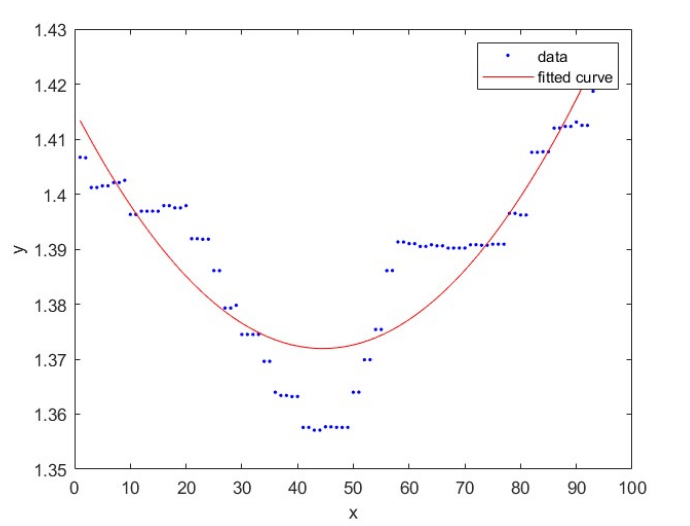
\includegraphics[width=7cm]{img/Face.png} }}%
\qquad
\subfloat[\centering NonFace]{{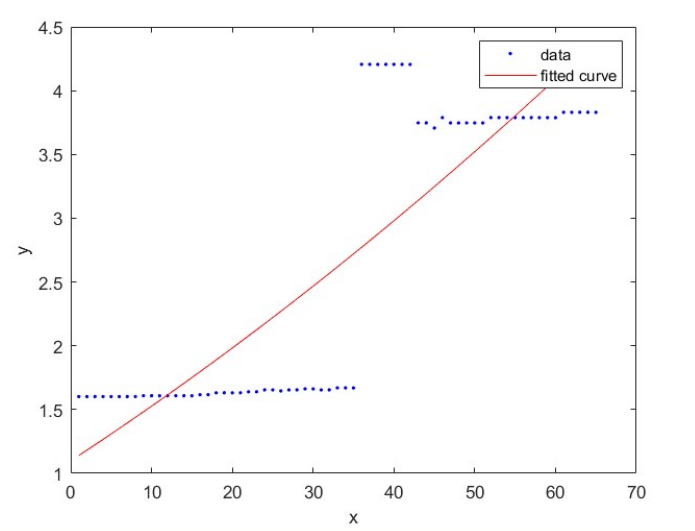
\includegraphics[width=7cm]{img/NonFacce.png} }}%
\caption{Confronto di Face e NonFace}
\end{figure}


Si nota inoltre che la parabola di una Face è giocoforza convessa.

Il marginRate è stato invece scelto sulla base del miglior compromesso
tra Precision e Recall.

\begin{figure}
\centering
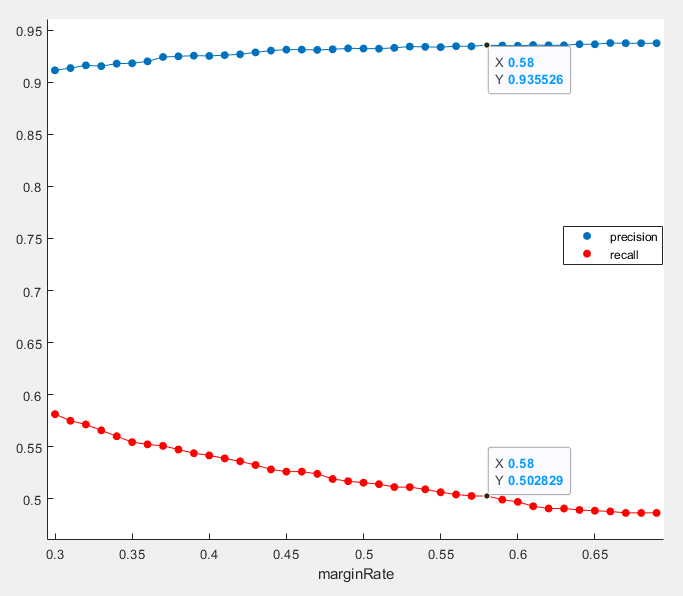
\includegraphics[width=\textwidth,height=0.31\textheight]{img/testingGraph.png}
\caption{Messa a confronto di Precision e Recall variando marginRate}
\end{figure}

Come si può vedere nel grafico all'aumentare del marginRate la Precision
aumenta a discapito del Recall.

E' stato scelto per questo come compromesso un marginRate di 0,58.

\pagebreak 

\hypertarget{pseudocodice}{%
\subsection{Pseudocodice}\label{pseudocodice}}

\begin{lstlisting}
Per ogni elemento con indice i di DepthDATA:
  matrix = DepthDATA{i}{2}; 
  fixedMatrix = FixMatrix(matrix);
  matrixVCenter = round(size(fixedMatrix, 1)/2);
  centralrow = fixedMatrix(matrixVCenter,:);
  f = parabolic_fit(centralrow);
  coefficientValues = coeffvalues(f);
  vertice = -coefficientValues(2)/(2 * coefficientValues(1)); // -b/2a
  marginRate = 0.58;
  matrixHCenter = round(size(fixedMatrix, 2)/2);
  marginA = matrixHCenter - marginRate*size(fixedMatrix, 1);
  marginB = matrixHCenter + marginRate*size(fixedMatrix, 1);
  
  if(vertice < marginA or vertice > marginB or coefficientValues(1) < 0):
      //contrassegno come NonFace
  else:
      //contrassegno come Face
\end{lstlisting}


\hypertarget{analisi-complessituxe0-temporale}{%
\section{Analisi Complessità
Temporale}\label{analisi-complessituxe0-temporale}}

Per analizzare la complessità del metodo si tiene conto della
complessità temporale delle seguenti funzioni utilizzate:

\begin{itemize}
\tightlist
\item
  size \(= O(1)\)
\item
  transpose \(= O(1)\)
\item
  fit \(= O(1)\)
\item
  max \(= O(n)\)
\end{itemize}

Per ognuna delle precedenti funzioni sono stati calcolati i vari tempi
di esecuzione al variare della quantità di dati utilizzati, i risultati
hanno portato alle precedenti conclusioni.

D'ora in avanti considereremo:

\begin{itemize}
\tightlist
\item
  n = numero di immagini
\item
  m = dimensione totale dell'immagine
\end{itemize}

Il metodo quindi ha complessità temporale pari a \(O(n \cdot m^2)\) in
quanto per ogni immagine viene calcolato il massimo una volta e poi
viene effettuato il controllo degli zeri sulla matrice, valore per
valore.

\hypertarget{risultati-e-prestazione-del-metodo}{%
\section{Risultati e Prestazione del
metodo}\label{risultati-e-prestazione-del-metodo}}

Il metodo ottiene quindi i seguenti risultati in termini di recall e
precision:

\(Precision = \frac{TruePositive}{TruePositive + FalsePositive} = \frac{711}{711+49} = 0.9355 \approx 94\%\)

\(Recalll = \frac{TruePositive}{TruePositive + FalseNegative} = \frac{711}{711+703} = 0.5028 \approx 50\%\)

Infatti vengono individuate correttamente 711 non Face con soli 49 falsi
positivi.

\pagebreak

\hypertarget{legenda-file}{%
\section{Legenda file}\label{legenda-file}}

\begin{itemize}
\tightlist
\item
  metodo1.m contiene l'effettivo programma che controllando tutte le
  immagini presenti dentro DepthDATA salva nel vettore results se è
  faccia (0.5) o non faccia (1)
\item
  checkResults.m a partire dal vettore results, conteggia il numero di
  NonFace correttamente individuate o erratamente individuate
\item
  fixMatrix.m contiene la funziona fixMatrix che data una matrice di
  profondità sostituisce i valori 0 con il massimo della profondità
\item
  testValori.m testa i vari valori di marginRate (da 0.3 a 0.7)
  calcolandone di volta in volta Precision e Recall. Alla fine mostra
  l'andamento del tutto
\item
  risultatiTestValori.fig mostra il grafico risultante dall'esecuzione
  del file testValori.m con l'andamento di Precision e Recall.
\end{itemize}

\end{document}
